\section{Contexte}

\subsection{Qu'est-ce que la réalité virtuelle ?}La notion de réalité virtuelle, contrairement à ce que l'on pourrait penser, n'est pas récente et date du début des années 80 quand Jaron Lanier, un informaticien américain pionnier du domaine, l'a popularisée. Cette notion n'a pourtant pas, à l'origine, l'exact sens qu'on lui prête habituellement aujourd'hui : une réalité virtuelle sous-entendrait qu'il s'agit d'une copie exacte de la réalité, ce qui n'est jamais le cas, faute de moyens techniques, et n'est pas toujours recherchée. Le terme venant  de l'anglais, \emph{virtual} peut se traduire par \emph{virtuelle} mais aussi par \emph{quasi} ou \emph{pratiquement}, or cette notion de \emph{quasi-réalité} correspondrait mieux à ce qu'est effectivement la réalité virtuelle. \\

En effet, de manière plus formelle, on peut définir la réalité virtuelle comme suit :

\begin{quote}\og \emph{La réalité virtuelle est un domaine scientifique et technique exploitant l'informatique et les interfaces comportementales en vue de simuler dans un monde virtuel le comportement d'entités 3D, qui sont en interaction en temps réel entre elles et avec un ou des utilisateurs en immersion pseudo-naturelles par l'intermédiaire de canaux sensori-moteurs.} \fg{}\end{quote}\cite{traiteRV1}

%Il faudra penser à citer la source : Le traité de la RV
Cela signifie que pour que l'on puisse parler de réalité virtuelle il faut que plusieurs conditions soient réunies :
\\
\begin{itemize}\renewcommand{\labelitemi}{$\bullet$}
\item \textbf{La présence d'interfaces comportementales et sensorielles. }
Les interfaces comportementales désignent les interfaces entre l'utilisateur et le monde virtuel. Il existe dans un premier temps des interfaces motrices, qui permettent de reconnaître les différentes actions que l'utilisateur peut entreprendre (mouvements, voix, etc). Ainsi le système informatique gérant le monde virtuel peut alors les prendre en compte. Les interfaces sensorielles font ensuite la liaison opposée et informent l'utilisateur de l'état du monde virtuel et des modifications éventuelles des actions entreprises précédemment (images, sons, etc). La réciprocité du besoin d'une interface motrice et sensorielle, qui sont nécessaires pour l'immersion du sujet et permettent de gérer l'interaction avec le monde virtuel, est illustrée par la \textsc{figure 1}.
\item \textbf{L'immersion du sujet.}
L'immersion caractérise le fait que les interfaces entre l'utilisateur et le monde virtuel doivent se faire oublier, et ce, en ressemblant le plus possible aux méthodes d'interaction que nous avons avec le monde réel. Elle ne peut pas être parfaite, car il y a toujours du matériel à utiliser qui n'est pas nécessaire pour interagir avec le monde réel (lunettes 3D, WiiMote, etc) mais doit être la plus totale possible.\\

\end{itemize}
\begin{figure}
  \caption{Interactions entre monde réel et virtuel \cite{traiteRV1}}
  %\centering
  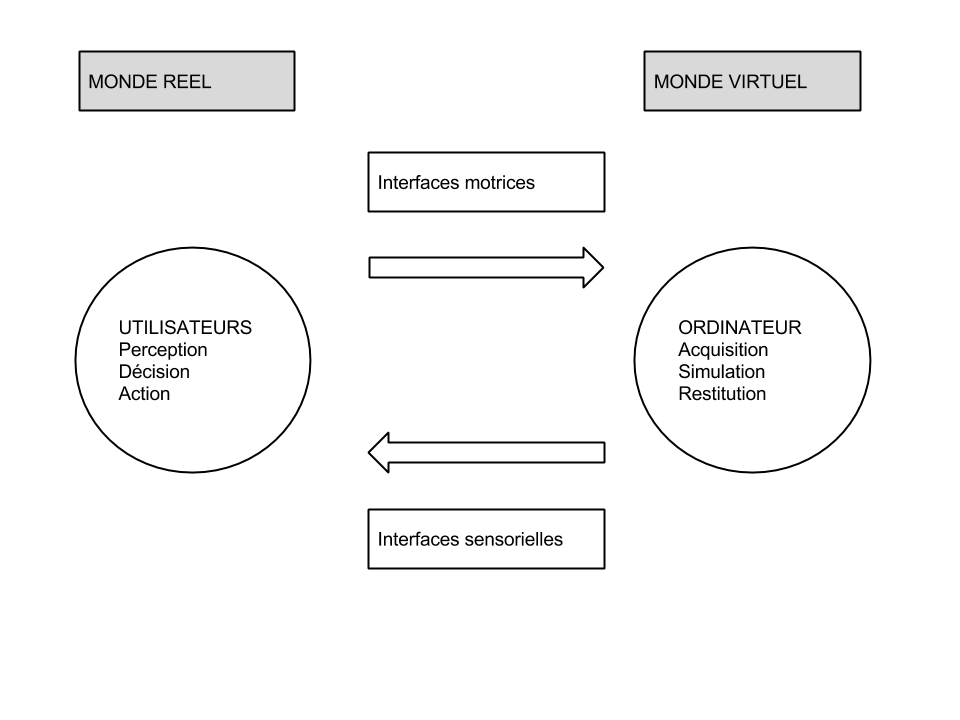
\includegraphics[scale=0.4,bb=0 0 720 720]{1-PreEtude/img/graphe_interfaces.png}
\end{figure}

La notion de réalité virtuelle implique donc également celles d'immersion et d'interaction, elles sont en fait constitutives de ce qu'est la réalité virtuelle. L'utilisateur doit pouvoir faire des actions motrices sur son environnement, il doit pouvoir agir dessus que ce soit par les mouvements, la parole, les gestes... Il n'y a pas de règles définies tant qu'il s'agit d'une activité motrice.
Une activité sensorielle, par ailleurs, signifie que l'utilisateur percevra un impact de ses actions sur le monde virtuel. Encore une fois il n'y a pas de liste de réponses sensorielles acceptables, ce peut être un son ou encore une modification de l'affichage.


\subsection{La Réalité Virtuelle et l'aide à la personne}

\subsubsection{L'aide à la personne}

Notre projet va traiter d'une application bien particulière de la réalité virtuelle (RV) : la santé. La RV est déjà utilisée dans le cadre de la santé et des soins. Les psychologues s'en servent par exemple pour traiter les cas de phobie, car une application de réalité virtuelle leur permet de plonger leurs patients dans la situation qui est l'objet de leur peur facilement, mais aussi de la garder sous contrôle et de la reproduire rapidement et à peu de frais. Le même avantage s'applique au traitement de l'autisme chez les enfants, car la RV permet de simuler des situations qui s'avéreraient dangereuses et qu'ils ne savent pas gérer, comme traverser une route seuls.\cite{traiteRV4}\\

Notre projet a été proposé par le centre de rééducation et de réadaptation fonctionnelle de Kerpape, et se focalisera donc sur le domaine d'expertise du centre, à savoir l'aide aux personnes handicapées. Le principe de l'aide à la personne est d'assister des personnes âgées ou handicapées dans les gestes de tous les jours, pour leur permettre de conserver leur autonomie.

\subsubsection{Le centre de Kerpape}

Nous avons eu l'occasion de visiter le centre de Kerpape au cours de notre projet. Kerpape accueille 400 patients chaque jour, et a pour objectif de leur permettre d'acquérir l'autonomie nécessaire à une réinsertion sociale et professionnelle. \\
Du fait de la grande diversité des handicaps que présentent les patients du centre, la modification du matériel existant est un pan important du travail de Willy Allègre et Jean-Paul Departe, les ingénieurs commanditaires de notre projet, et cela rend la RV particulièrement intéressante, un logiciel étant plus facilement reconfigurable que du matériel.\cite{kerpape}\\


C'est le second projet de RV auquel participe le centre de Kerpape. Le premier était le projet AGATHE, débuté en 2009, dont le but est d'aider les personnes atteintes de troubles cognitifs (par exemple dus à la maladie d'Alzheimer, à des AVC, ...) à être autonomes dans la vie de tous les jours. Le projet consiste en la réalisation d'un \og voisinage virtuel \fg{} dans lequel le patient peut se déplacer, et où se trouvent plusieurs points d'intérêts avec lesquels il peut interagir, tel qu'un bureau de poste, un supermarché, etc. Le patient a donc accès à différentes actions en accord avec le lieu dans lequel il se trouve, et le thérapeute peut évaluer ses performances en fonction de plusieurs critères comme le temps passé par le patient dans une zone donnée.\cite{agathe}

\subsubsection{Le projet Avalon}

Le projet qui nous a été confié, le projet Avalon, est le premier projet de collaboration entre Kerpape et l'INSA. Il a aussi pour but d'aider les personnes handicapées à recouvrer leur autonomie, mais il se focalise sur un aspect différent de la vie de tous les jours : l'utilisation de la domotique dans l'habitat des patients. Durant leur phase de rééducation au centre de Kerpape, les patients sont amenés à vivre quelques temps dans un appartement \enquote{tremplin} appartenant au centre. Ces appartements sont lourdement équipés en domotique pour que des personnes handicapées puissent y être autonomes, les différentes portes, fenêtres et volets sont contrôlables à distance par différents interrupteurs, un plan de travail dans la cuisine est réglable en hauteur, un mobile accroché à des rails au plafond aide les déplacements, etc.
Les appartements tremplins servent à présenter aux patients les différents équipement disponibles pour leur propre appartement une fois qu'ils quitteront le centre, mais aussi à les entraîner à l'usage de ces équipements, qui peut s'avérer complexe, particulièrement pour les personnes souffrant de handicaps mentaux. \\

Le centre de Kerpape a donc initié le projet Avalon pour permettre aux patients de se préparer à l'utilisation des appartements même si ceux-ci sont occupés, et pour que les thérapeutes encadrant les patients puissent profiter de différents modes d'utilisation leur permettant de se focaliser sur les interactions les plus problématiques, comme détaillé dans le cahier des charges.
